Mit geoelektrischen Messungen werden Materialeigenschaften wie die Ionenkonzentration, Grad der Wassersättigung und der Permeabilität untersucht. 
Das bedeutet, dass mit Hilfe dieses Verfahrens z.B der Grundwasserspiegel bestimmt werden kann.

Bei den Messmethoden wird zwischen aktiven und passiven Verfahren unterschieden.  Da sowohl bei der Schlumberger-Sondierung als auch bei der Wenner-Kartierung eine Spannung angelegt wird, werden die beiden Verfahren zu den aktiven Messmethoden gezählt.

Während der Geländeübung werden die Messungen mit dem Wechselstromverfahren durchgeführt. Dabei wird an zwei Elektroden Wechselstrom angelegt,
über zwei Sonden an der Oberfläche wird die Spannung gemessen. Mit diesem Verfahren wird also die Materialeigenschaft, elektrischen Strom zu leiten, untersucht.

Hierbei unterscheidet man zwischen elektrischer Leitfähigkeit, wenn Elektronen bewegt werden, und ionischer Leitfähigkeit, dem Transport von Ionen. 
Aufgrund der elektrischen Leitfähigkeit können z.B Metallrohre im Boden lokalisiert werden. Ionische Leitfähigkeit tritt in Gesteinen und Lockersedimenten auf,die einen entsprechenden Wassergehalt haben.

Als Materialeigenschaft wird der spezifischen Widerstand $$[\rho] = \SI{1}{\Omega m}$$ bestimmt. Er ist der Kehrwert der Leitfähigkeit $\sigma$. Je nach Material und Wassergehalt variieren diese Werte. Es wird ein Strom in die Erde eingespeist und anhand des Spannungsabfalls, der mit Hilfe der Sonden gemessen wird, wird auf den Widerstand der stromdurchflossenen Materialien geschlossen. Während der Geländeübung wird ein Basaltgang untersucht. Basalt hat einen relativ hohen spezifischen Widerstand, sodass er durch ein Ansteigen  von $ \rho$ lokalisiert werden kann.

Die Formeln und Methodenbeschreibungen wurden in \cite{skript} nachgelesen.

\section{Schlumberger-Anordnung}

Die Schlumberger-Anordnung wird in der Geländeübung zur Sondierung verwendet. Es wird die Änderung des spezifischen Widerstands in den verschiedenen Schichten des Untergrunds unter einem bestimmten Punkt bestimmt. In Abbildung \ref{abb:Schlumberger} ist die Schlumberger-Anordnung schematisch dargestellt. Der Ort, an dem gemessen wird, ist der Mittelpunkt der Anordnung. Um in verschieden Tiefen Messwerte zu erhalten wird der Abstand zwischen den Elektroden und den Sonden jeweils symmetrisch erhöht. Sinnvoll ist es, den Abstand exponentiell zu erhöhen und ein Profil mit möglichst wenig Topographie zu wählen.

%%%%%%%%%%%%%%%%%%%%%%%%%%%%%%%%%%%%%
\begin{figure}[ht]
\centering
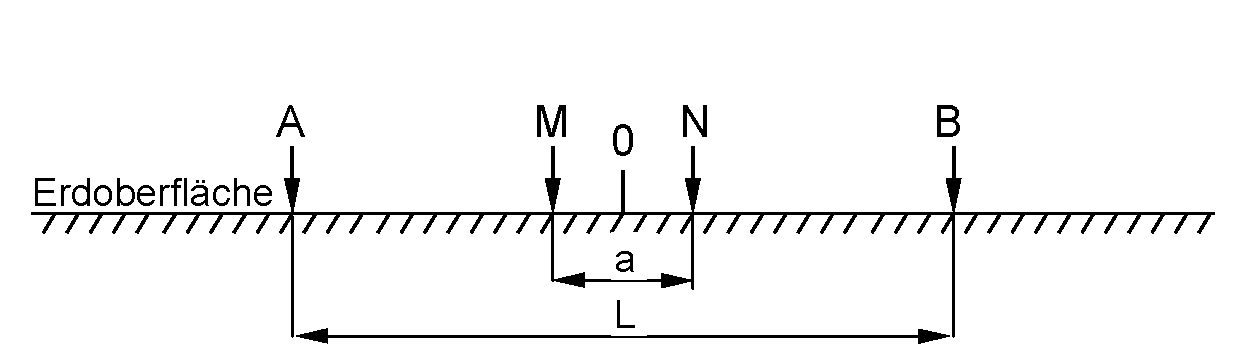
\includegraphics[width=0.6\textwidth]{Schlumberger.png}
\caption{Schematische Darstellung der Schlumberger-Anordnung}
\label{abb:Schlumberger}
\end{figure}
%%%%%%%%%%%%%%%%%%%%%%%%%%%%%%%%%%%%

Beim Stecken der Stromelektroden ist es wichtig eine möglichst große Kontaktfläche zu haben, da es an diesen zu Kontaktwiderstand kommt. Eine große Kontaktfläche erreicht man, indem man die Stromelektroden möglichst tief in die Erde steckt. 
Das gleiche gilt natürlich für die Wenner-Kartierung.

\section{Wenner-Kartierung}

In Abbildung \ref{abb:Wenner} ist der schematische Aufbau der Wenner-Anordnung zu sehen. Bei \textbf{A} und \textbf{B} sind die Elektroden und bei \textbf{M}, \textbf{N} die Sonden zur Spannungsmessung.

%%%%%%%%%%%%%%%%%%%%%%%%%%%%%%%%%%%%%
\begin{figure}[ht]
\centering
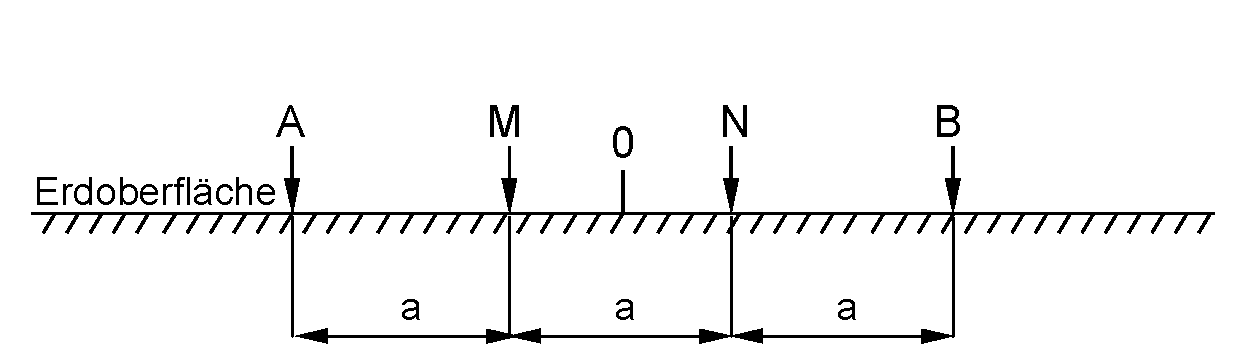
\includegraphics[width=0.6\textwidth]{Wenner.png}
\caption{Schematische Darstellung der Schlumberger-Anordnung}
\label{abb:Wenner}
\end{figure}
%%%%%%%%%%%%%%%%%%%%%%%%%%%%%%%%%%%%

Bei der Wenner-Kartierung werden die Abstände zwischen den Elektroden konstant gehalten und die ganze Anordnung wird über den Boden verschoben. Somit wird in einer Tiefe an verschieden, horizontal versetzten Punkten im Untergrund gemessen. Der Abstand $a$ der Elektroden entspricht auch der Tiefe, in der die Messung durchgeführt wird.
Hierbei muss aber bedacht werden, dass oben liegende, sehr gut leitende Schichten den Strom bündeln und somit zu einem verfälschten Messergebnis führen können.

\section{Geoelektrische Tomographie}
Die Tomographie ist eine Mischung aus der Wenner-Kartierung und Schlumberger-Sondierung. Die Wenner-Kartierung wird praktisch in verschiedenen Tiefen durchgeführt und über eine Profil bewegt, dadurch wird ein zweidimensionales Bild des Untergrunds erstellt.
Mit Hilfe eines Computerprogramms kann durch Inversion der gemessenen Werte ein Modell für die Verteilung des spezifischen Widerstands im Untergrund erstellt werden.

\section{Spezifischer Widerstand und Geometriefaktor}
\label{sec:spezW}

Die Potentialdifferenz bei einem angelegten Strom $I$ ist
\begin{equation}
V = \rho \, I \, \frac{1}{2 \pi} \big(\frac{1}{r_{\mathrm{AM}}} - \frac{1}{r_{\mathrm{MB}}} + \frac{1}{r_{\mathrm{NB}}} - \frac{1}{r_{\mathrm{AN}}} \big) \, ,
\end{equation}
wobei mit $r_{\mathrm{AM}}$ usw. jeweils die Abstände zwischen den Sonden und Elektroden, wie in Abbildung \ref{abb:Wenner} zu sehen, bezeichnet werden.
Um den spezifischen Widerstand leichter berechnen zu können, wird der Geometriefaktor
$$F = \frac{2 \pi}{\frac{1}{r_{\mathrm{AM}}} - \frac{1}{r_{\mathrm{MB}}} + \frac{1}{r_{\mathrm{NB}}} - \frac{1}{r_{\mathrm{AN}}}}$$
eingeführt.
Damit lässt sich $\rho$ berechnen mit 
\begin{equation}
\rho = \frac{V}{I} \, F.
 \label{eq:roh}
\end{equation}

\textbf{Scheinbarer spezifischer Widerstand}

Ist der Untergrund nicht homogen, wird der Wert der Formel \eqref{eq:roh} als scheinbarer spezifischer Widerstand bezeichnet. Der Geometriefaktor hängt nur von der geometrischen Anordnung ab und nicht von der 
Leitfähigkeit des Untergrunds, weshalb der scheinbare spezifische Widerstand $q_a$ nur im Falle eines homogenen Untergrunds gleich dem spezifischen Widerstands ist.\\
Im Falle der Wenner-Anordnung wird  der scheinbare spezifische Widerstand mit der Formel
$$ \rho_a = 2 \pi \frac{V}{I} a $$
berechnet.
Bei einer Messung wird versucht, durch Interpretation der gemessenen scheinbaren Widerstände den spezifischen Widerstand zu finden.